\documentclass[border=3mm]{standalone}

\usepackage{tikz}
\usetikzlibrary{arrows.meta}

\begin{document}
	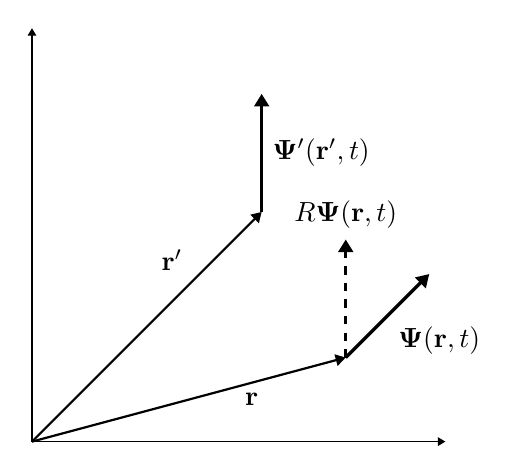
\begin{tikzpicture}[scale=1.5]
		\draw[-{Triangle[scale=0.75]}] (0,0) coordinate (o) -- (3.5,0);
		\draw[-{Triangle[scale=0.75]}] (o) -- (0,3.5);
		\draw[thick,-{Triangle[scale=0.75]}] (o) --++ (15:2.75cm) coordinate[pos=.5] (a) node[pos=0.7,below]{$\mathbf{r}$} coordinate (1);
		\draw[thick,-{Triangle[scale=0.75]}] (o) --++ (45:2.75cm)node[pos=0.7,above left]{$\mathbf{r'}$} coordinate (2);
		\draw[very thick,-{Triangle[scale=0.75]}] (1) --++ (45:1cm) node[midway,below right] {$\mathbf{\Psi(r},t)$};
		\draw[very thick,-{Triangle[scale=0.75]},dashed] (1) --++ (90:1cm) node[above] {$R\mathbf{\Psi(r},t)$};
		\draw[very thick,-{Triangle[scale=0.75]}] (2) --++ (90:1cm) node[midway,right] {$\mathbf{\Psi'(r'},t)$};
	\end{tikzpicture}
\end{document}